
We examine the importance of contextual congruence by exploring the semantic distance between text and image modalities and whether utilizing external knowledge from ConceptNet will bring this distance closer and better reflect their semantics, as explained below. More specifically, we measure contextual congruence in multimodal content using the semantic distance between the separate image and caption (text) representations, as this distance is expected to be shorter in a relatively congruent multimodal representation \cite{mandera2017explaining,frank2017word,beck2011congruence,maki2004semantic}. We can then demonstrate how external knowledge can enhance and contextualize the representations to bridge the semantic gap between the modalities. In doing so, we can better predict the success of crowdfunding campaigns. 


We generated the captions for image modality using BLIP to demonstrate this idea, resulting in a textual description for each modality as text. We used semantic search (see Section Knowledge Retrieval) to extract the most relevant concepts for both text and image captions. Then, we appended these concepts to the input, which is a pair of text and image captions, to generate representations using BERT. We performed clustering analysis using DB-SCAN over the text and image captions --- we validated that the clusters represented text and image modalities.--- Our goal here is to show how the centroids of each cluster change when external knowledge is included in the input. Hence, we ran two clustering algorithms, with and without external knowledge.

\begin{figure}[hbt!]
\vspace{-1.1em}
  \centering
  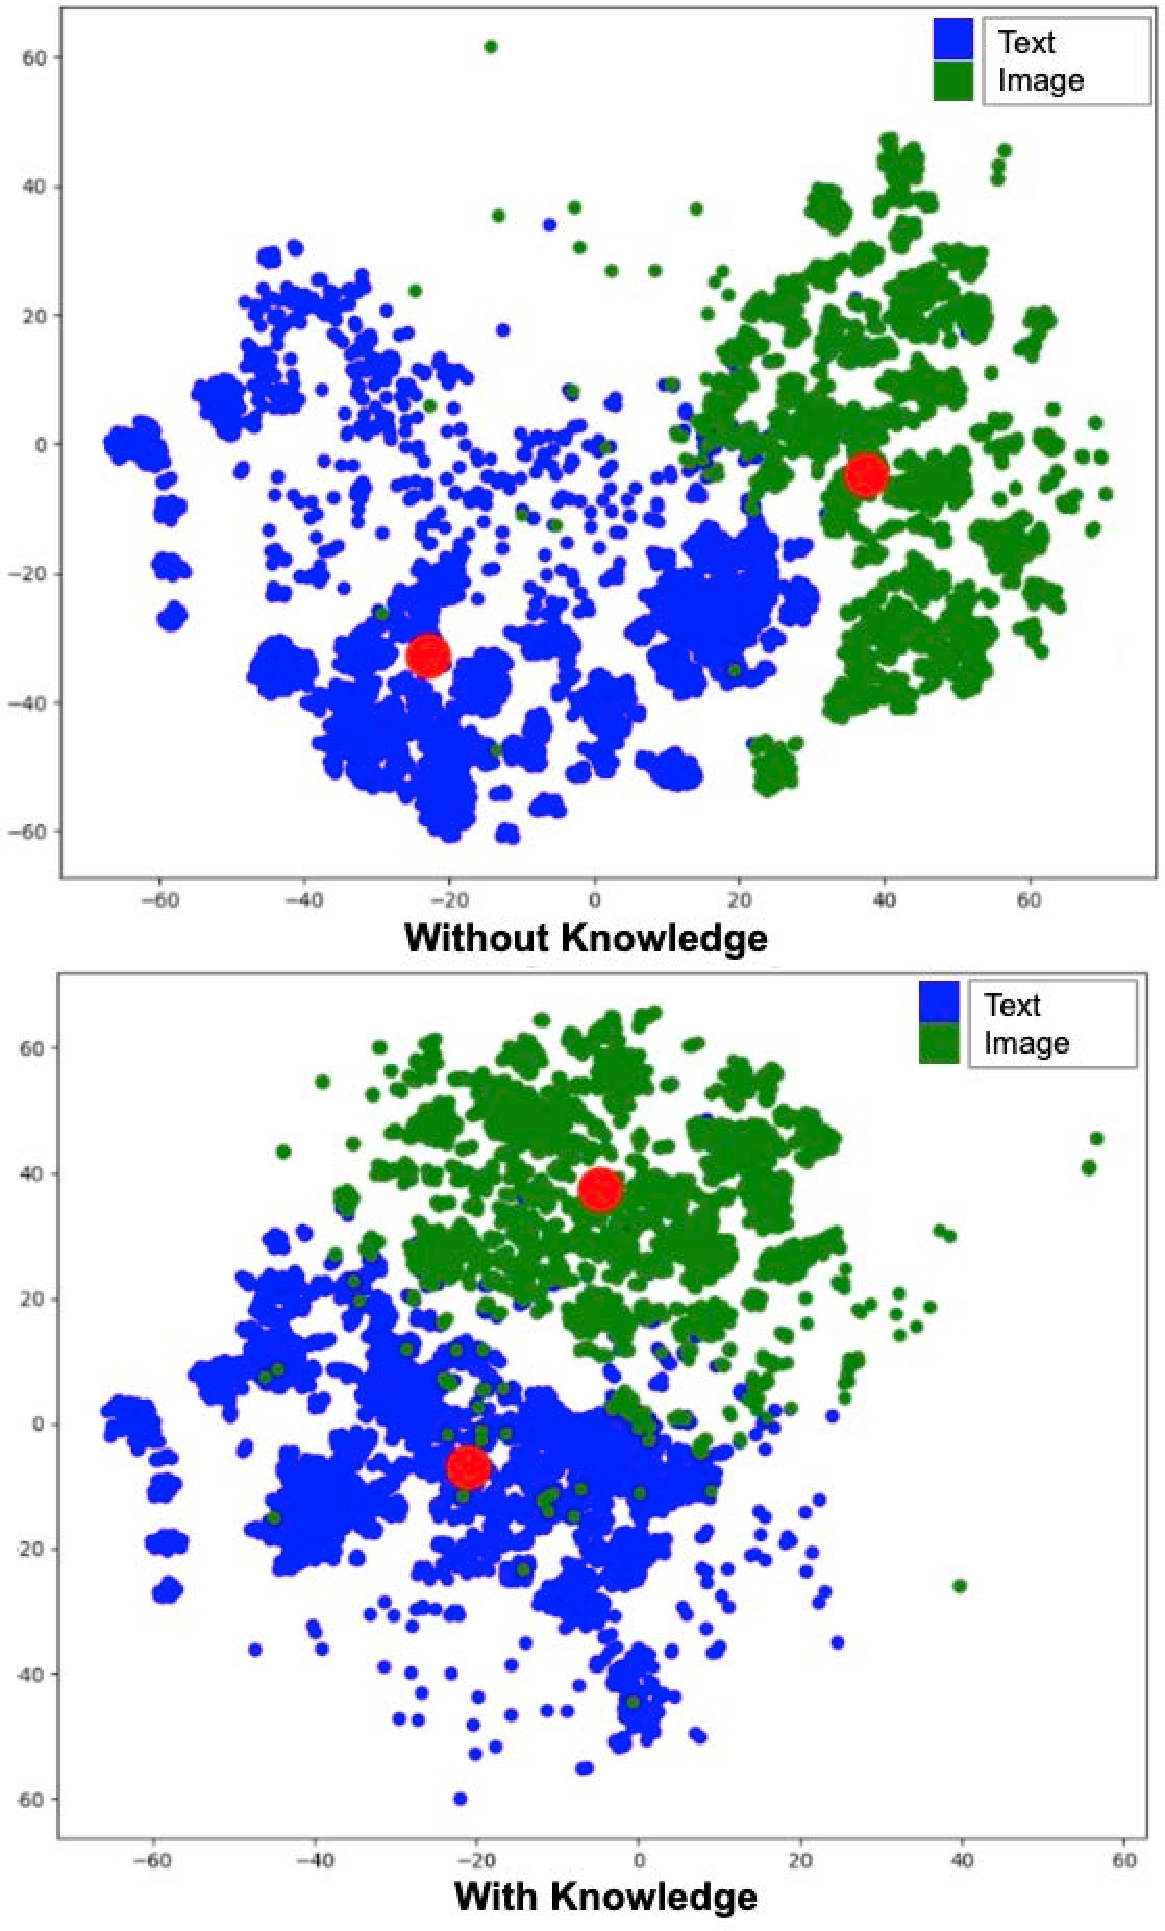
\includegraphics[width=8cm]{Figures/congruence_cluster_vertical.pdf}
\vspace{-1.5em}
\caption{t-SNE visualization of text and image caption (BLIP) embeddings as two clusters. The red dots represent the centroids in each cluster. The two clusters get denser and the distance between the text and image clusters reduces when we include concepts that we extracted from ConceptNet based on text and image captions.}
\vspace{-1.2em}
\label{fig:embds-cluster}
\end{figure} 


Figure \ref{fig:embds-cluster} shows t-SNE visualizations of the text and image clusters created with and without external knowledge. The upper clusters (without knowledge) are more scattered, whereas the lower clusters are denser. The centroids in the clusters with knowledge are also closer to each other, demonstrating the semantic distance is reduced because it can better reflect their semantic relationships. We ran the same experiment with different sizes of data points; 
%and our observation did not change as 
the clusters consistently got denser and centroids closer (see Figure \ref{fig:context_congruence_across_data_size} in the Appendix).
We also measured semantic similarity using cosine for each text-image pair in these clusters and created their density plots (see Figure \ref{fig:density-plot}). 
%In other words, rather than measuring the semantic distance between centroids, we measured the similarity between image and text modalities in a pair. From figure 
Figure \ref{fig:density-plot} shows
%we can also observe that 
that the similarity between text and image modalities increased by about 9.9\%.


\begin{figure}%[hbt!]
  \centering
  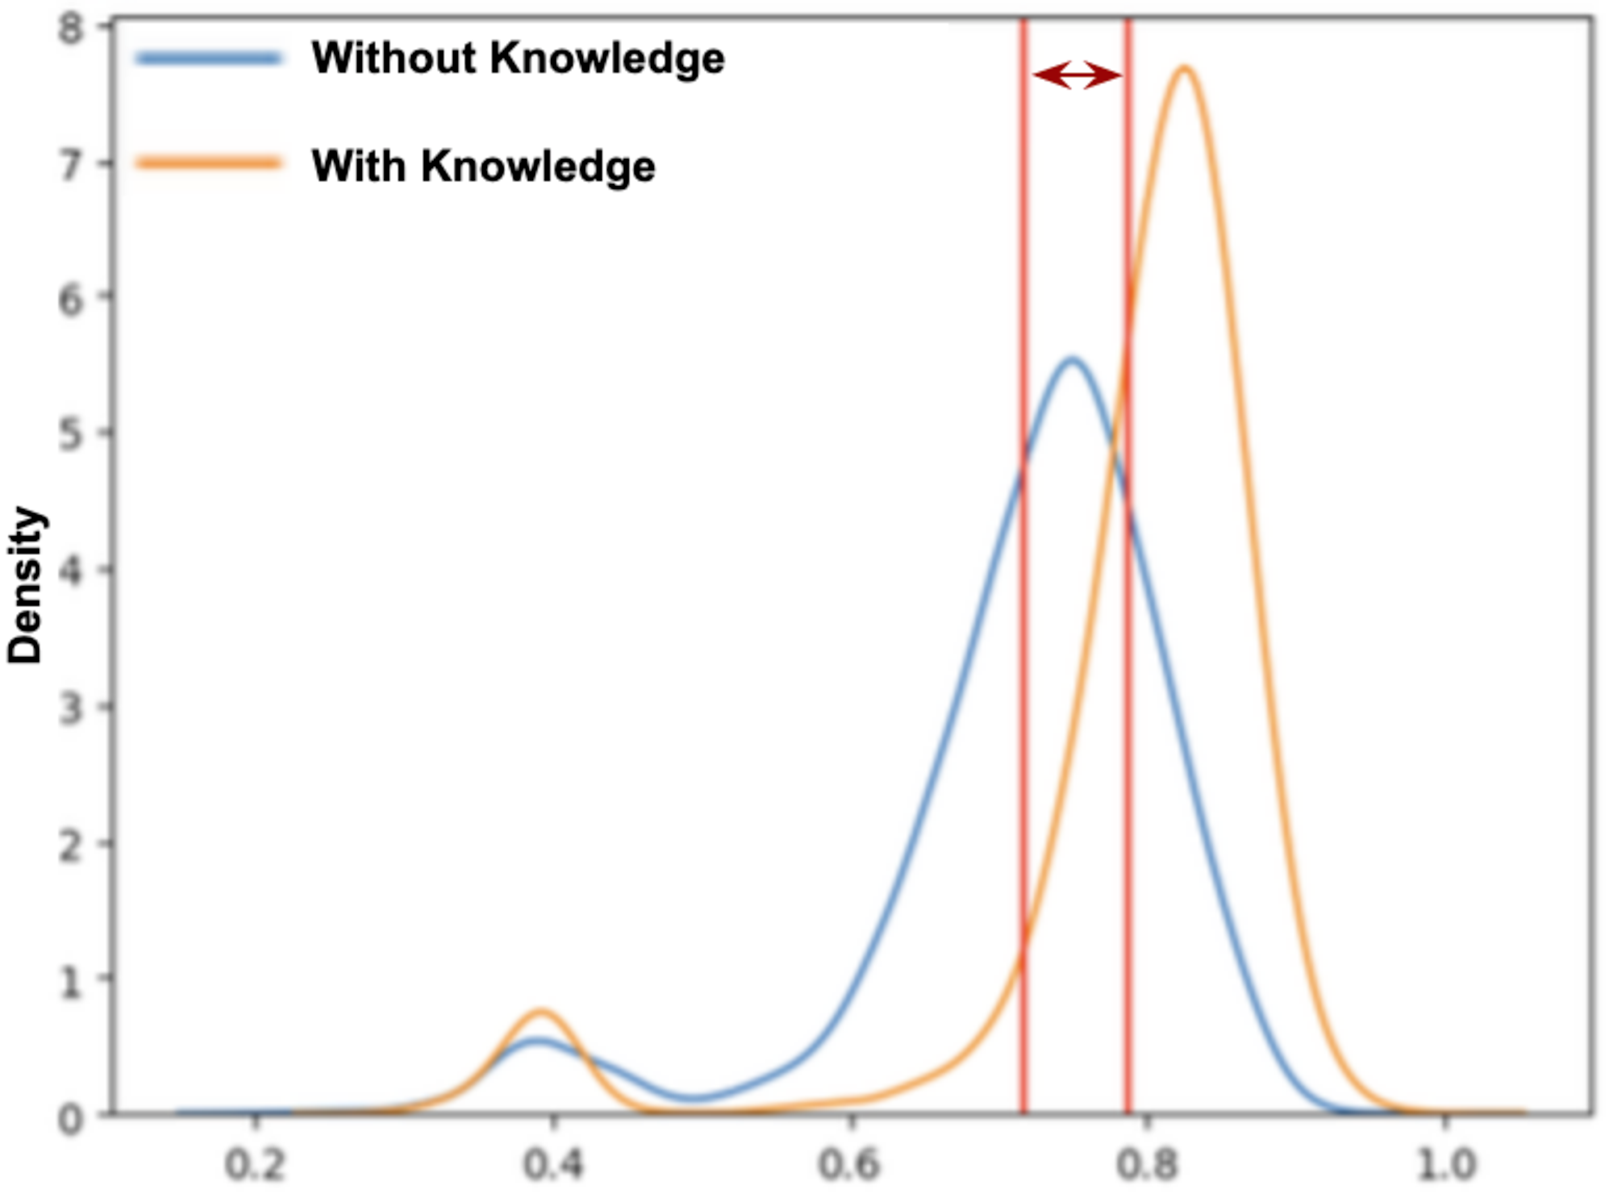
\includegraphics[width=7.8cm]{Figures/density-plot.pdf}
\vspace{-1em}
\caption{Density Plot demonstrates the difference between the similarities (cosine) of the image and text embeddings with and without knowledge. The inclusion of knowledge in the input gets text and image modalities closer by about 9.9\%.}
\vspace{-2.3em}
\label{fig:density-plot}
\end{figure} 


In addition, as we pair image and text modalities (see Figure \ref{fig:image-womens-movement-patriachy}),
% with the 
%human-generated 
% caption, 
the VLMs recognize relationships between modalities. %capturing the meaning to an extent while 
However, hallucinations are amplified by making non-existent connections and nonfactual information. Explicit knowledge from KGs can facilitate 
%the contextualizing and 
factual grounding.
%to capture the true meaning. 
We queried the KG to extract relevant concepts and simply include these with the pair of images and text as input for the VLMs such as Llava and BLIP. 
%We observe that the hallucinations are mitigated. 
This mitigates hallucinations. 
%For instance, in our example in 
As shown in Table \ref{tab:generated-caption-two-women}, the generated caption with knowledge does not include hallucination while containing contextual relationships from both the image and human caption.
%and is more contextually meaningful as the image and human caption are embedded in the meaning. The reader may find more 
Other examples appear in the appendix with generated captions (see Table \ref{tab:generated-captions}). 
These observations demonstrate the potential contribution of external knowledge to create more congruent multimodal representations by forming contextual relationships between modalities.  


\begin{figure*}[hbt!]
 % \vspace{-4em}
    \centering
  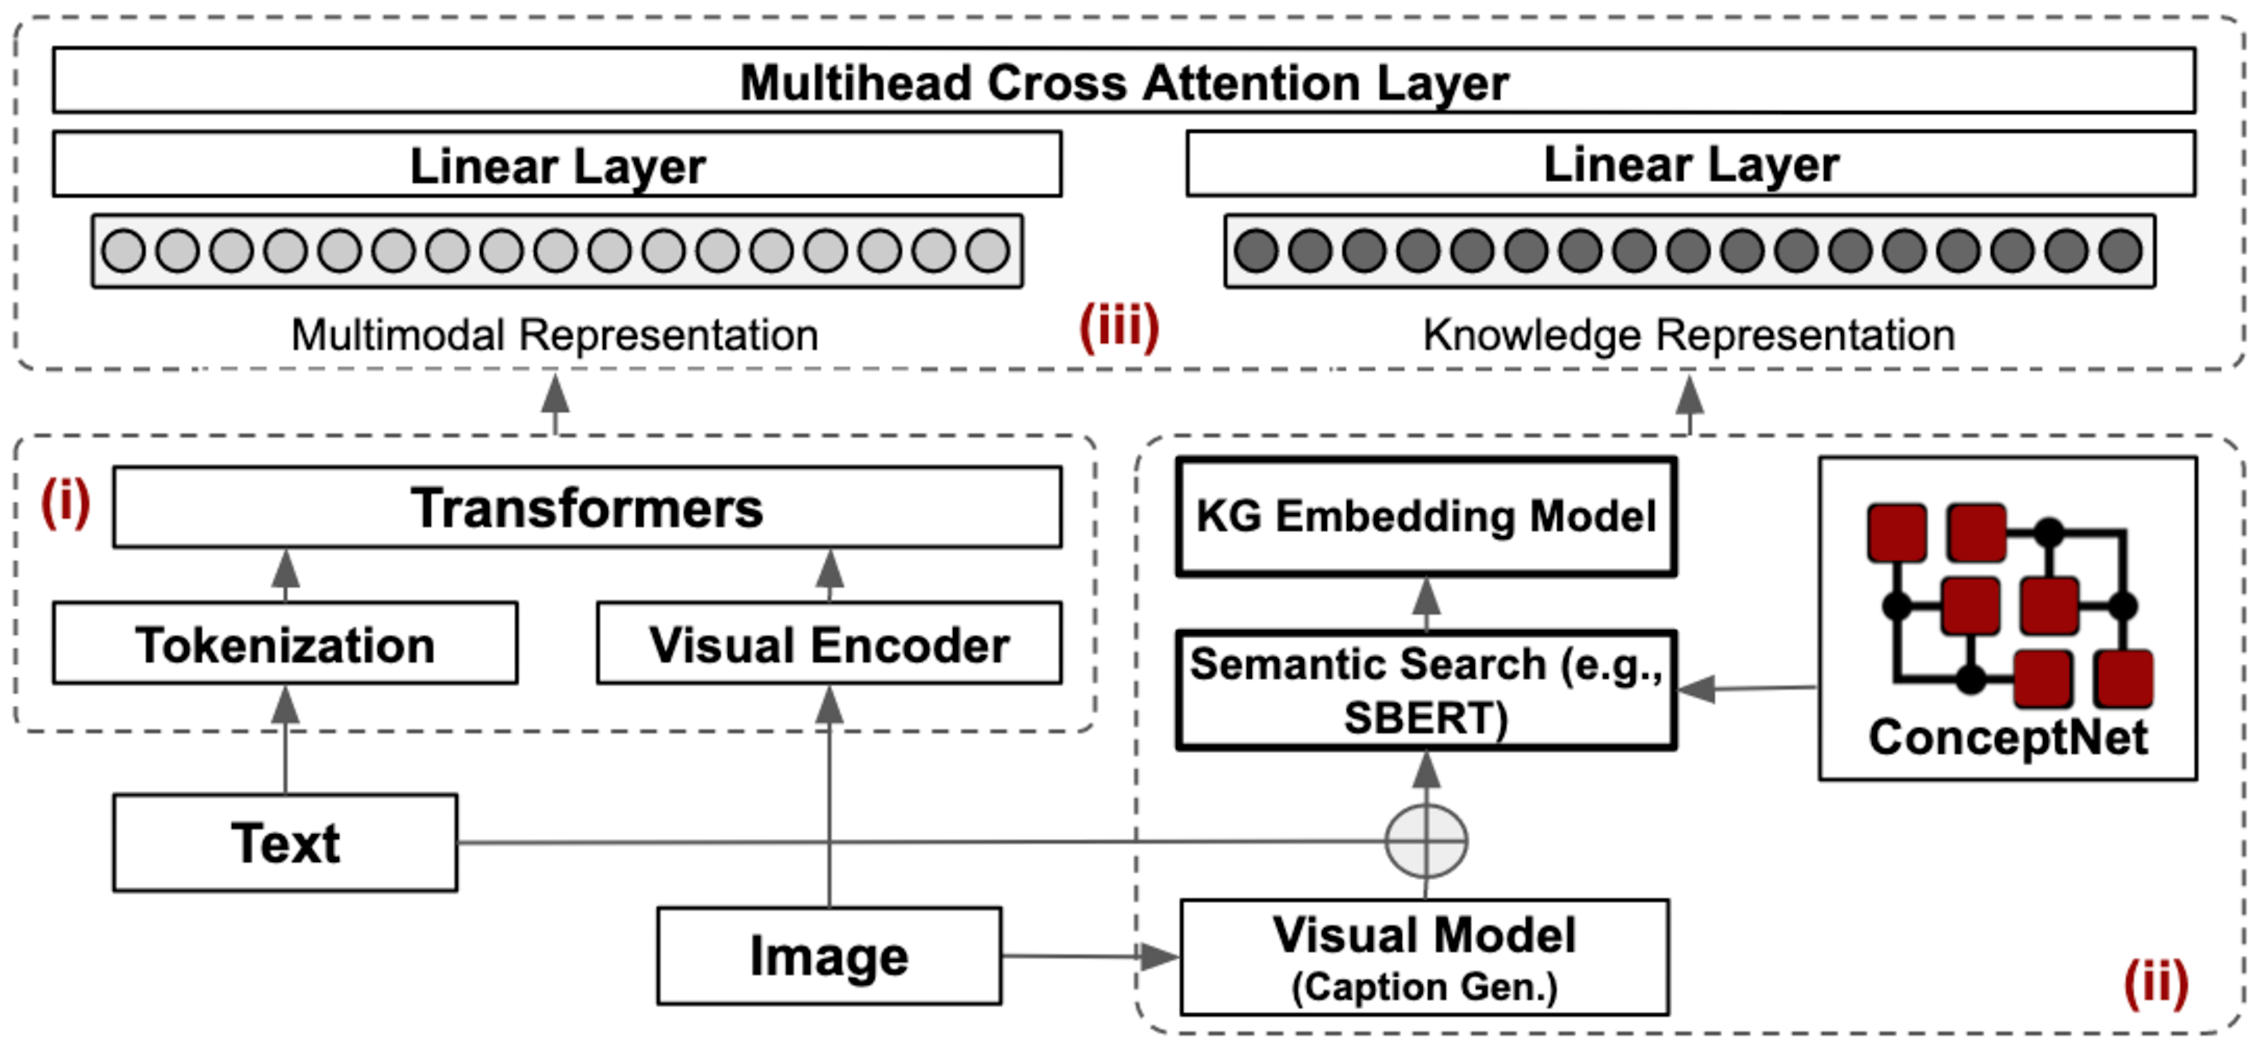
\includegraphics[width=17cm]{Figures/diagram.pdf}
\vspace{-0.8em}
\caption{Our approach consists of three main components: (i) multimodal learning, (ii) knowledge retrieval and representation, and (iii) Knowledge Fusion Layer. The Retrieval component identifies the most relevant concepts from ConceptNet. The concepts' KG embeddings are generated. The knowledge fusion layer fuses the multimodal representations with knowledge embeddings followed by Softmax.}
\vspace{-1em}
\label{fig:architecture}  
\end{figure*}